% !TEX encoding = UTF-8 Unicode
\documentclass{01_preamble/classicreport}
% big font for sections
%\usepackage{sectsty}
%\sectionfont{\LARGE}

\usepackage{graphicx}
\usepackage{wrapfig}
\usepackage[labelfont={bf,sf}]{caption}
\usepackage{subcaption}
\usepackage{listings}
\usepackage{hyperref}
\usepackage{blindtext}




\title{Classic theme template}

\author[a]{Navn Navnsen}
\author[b]{Navn Andetnavnsen}
\affil[a]{navn@navnsen.com} 
\affil[b]{navn@andetnavnsen.com}

\dates{\today}
	
% REFERENCES SETUP
\usepackage[round, authoryear]{natbib}
\bibliographystyle{humannat}

% SET TITLES OF CONTENTS AND REFERENCES
\addto\captionsenglish{% Replace "english" with the language you use
  \renewcommand{\contentsname}%
    {Table of Contents}%
}
\renewcommand{\refname}{References}

\begin{document}

\maketitle
\thispagestyle{empty}
\vskip24pt
\begin{abstract}
\noindent
% !!!!!!!!!!!!!!!!!!!!!! CONTENT HERE
\blindtext
\end{abstract}
\vskip24pt

% COMMENT NEXT LINES TO REMOVE TABLE OF CONTENTS
% \pagebreak
% \tableofcontents
% \listoffigures
% \listoftables
% \pagebreak 

\dropcap{L}{etter which} is lowered here, also a cite \citep{christensen_assessing_2015}.
\blindtext[4]
\begin{quote}{Richard P. Feynman}
    \enquote{\textit{Fall in love with some activity, and do it! Nobody ever figures out what life is all about, and it doesn't matter. Explore the world. Nearly everything is really interesting if you go into it deeply enough. Work as hard and as much as you want to on the things you like to do the best. Don't think about what you want to be, but what you want to do. Keep up some kind of a minimum with other things so that society doesn't stop you from doing anything at all.}}
\end{quote}

\noindent\blindtext[2]

\begin{equation}
   \int_{\mathbb{R}} \frac{\partial f(y_i|\theta)}{\partial \theta} \frac{\partial f(y_i|\theta)}{\partial \theta} f(y_i|\theta) 
    + \frac{\partial^2 \log f(y_i|\theta)}{\partial \theta \partial \theta'}f(y_i|\theta) = 0
\end{equation}

\blindtext
%=================
\section{Some section}
\dropcap{h}{ere is} some more content.
% !!!!!!!!!!!!!!!!!!!!!! CONTENT HERE
\blindtext 
\citep{alyass_big_2015}

\subsection{this is a subsection}
\blindtext[2]
\subsubsection{This is a subsubsection}
\blindtext
\subsubsection{This is another subsubsection}
\blindtext
\begin{equation}
    Y = B\cdot K^\alpha L^{1-\alpha}
\end{equation}


\section{Another section}
\dropcap{W}{hat about} some more content.
\blindtext[2]

\begin{wrapfigure}{r}{0.6\textwidth}
    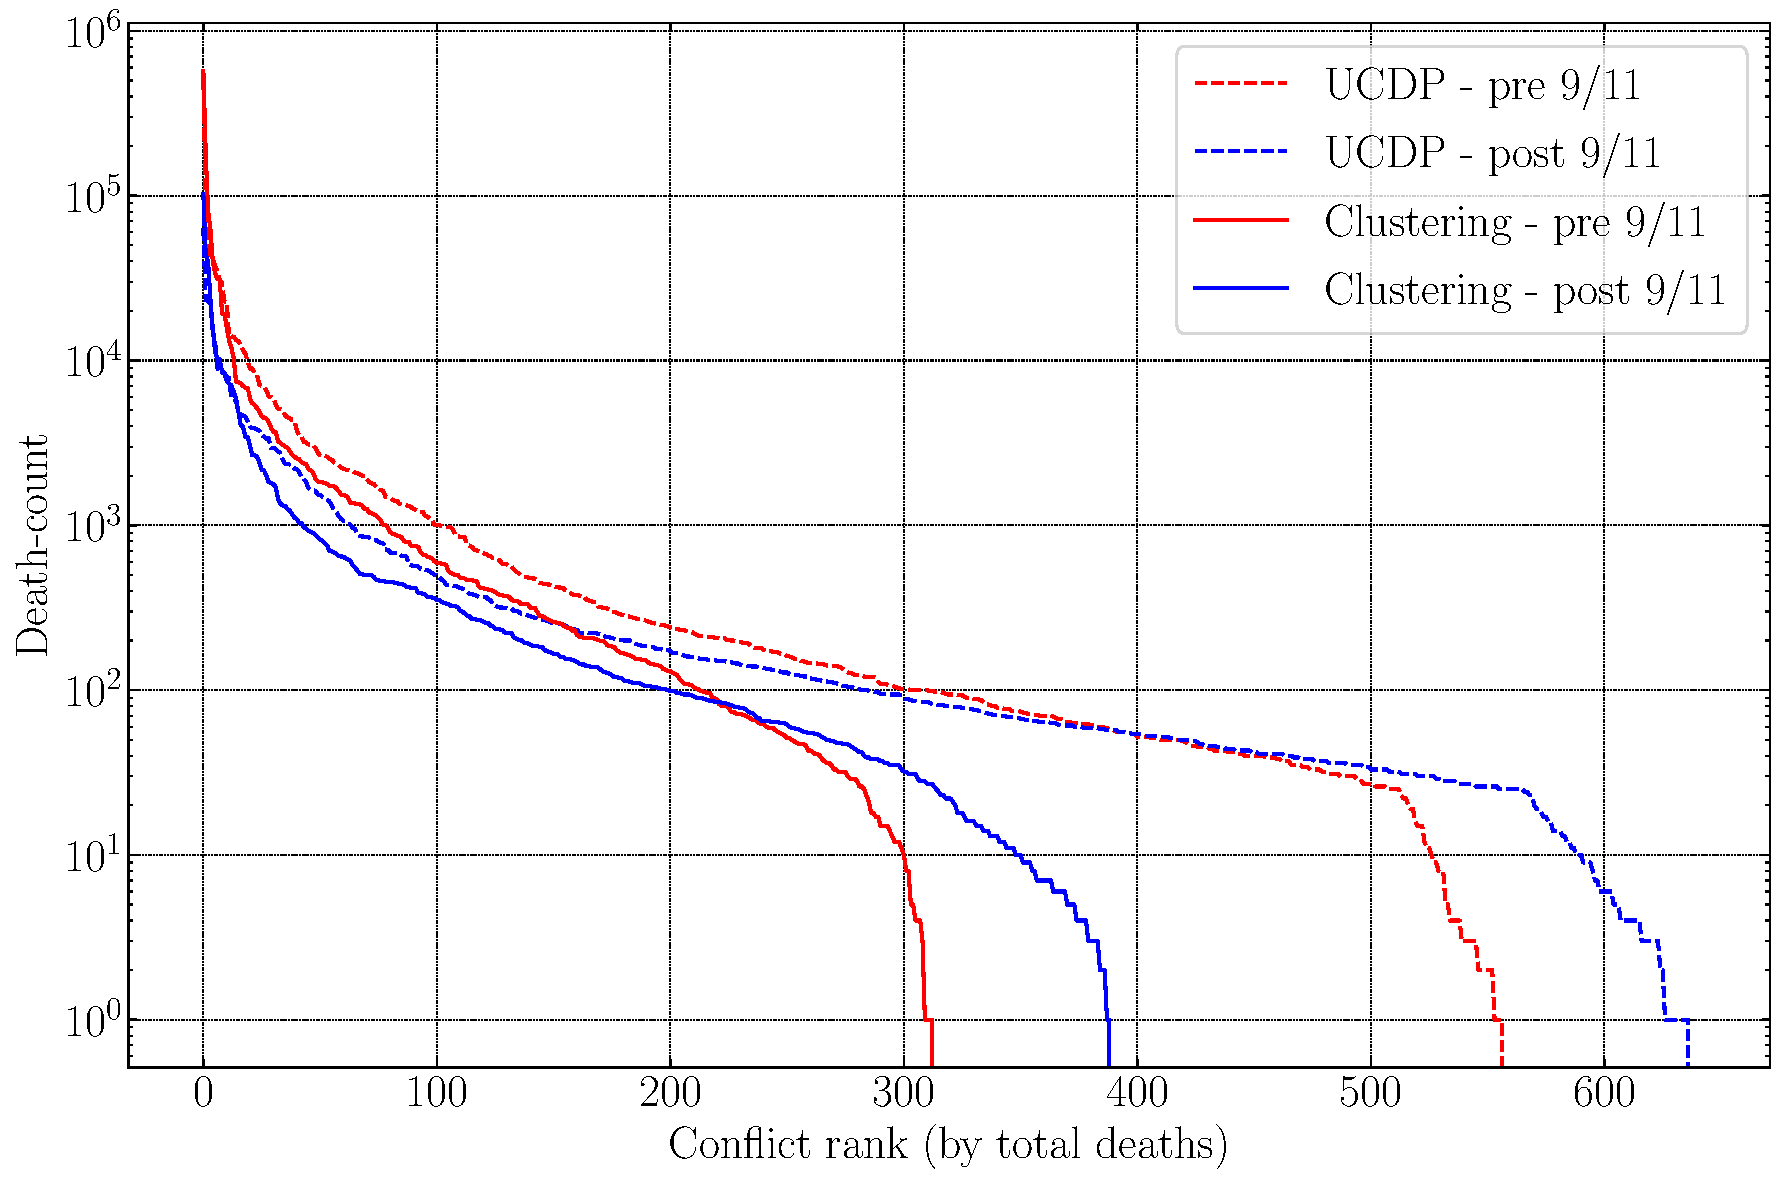
\includegraphics[width=0.6\textwidth]{02_figures/deathcomparison.pdf}
    \caption[This is something]{This is something with a really long caption text describing what you're looking at.}
\end{wrapfigure}

\blindtext[5]

\newpage
% CHANGE THIS IF YUOR BIBFILE HAS A DIFFERENT NAME
{\small
\bibliography{references.bib}
}
\end{document}
